\documentclass[12pt,a4paper]{article}
\usepackage[a4paper,top=1.5cm, bottom=1.5cm, left=1.5cm, right=1.5cm]{geometry}
\usepackage[T2A]{fontenc}
\usepackage[utf8]{inputenc}
\usepackage[russian]{babel}
\usepackage{amsmath}
\usepackage{amssymb}
\usepackage{graphicx}
\usepackage{floatrow}
\usepackage{booktabs}
\usepackage{wrapfig}
\usepackage{indentfirst}
\usepackage{lipsum}
\usepackage{subcaption}
\usepackage{float}
\usepackage{enumitem}
\restylefloat{table}

\newcommand{\figref}[1]{(см. рис. \ref{#1})}
\newcommand{\e}[1]{\text{$\cdot10^{#1}$}}

\author{\normalsize Симанкович Александр, Дедков Денис
	\\ \normalsize группа Б01-108 \\
	\normalsize 22.10.2022}
\date{}

\usepackage{float}
\restylefloat{table}
\title{
	\large Отчет о выполнении лабораторной работы \\
	\Large <<Цифровой осциллограф>> \\ 
	
}

\begin{document}
\maketitle
\newpage
\section*{1. Спектр дискретизованной синусоиды}
\subsection*{1.2. Спектр дискретизованной синусоиды (окно Ханна)}
\vspace*{20pt}

\begin{center}
	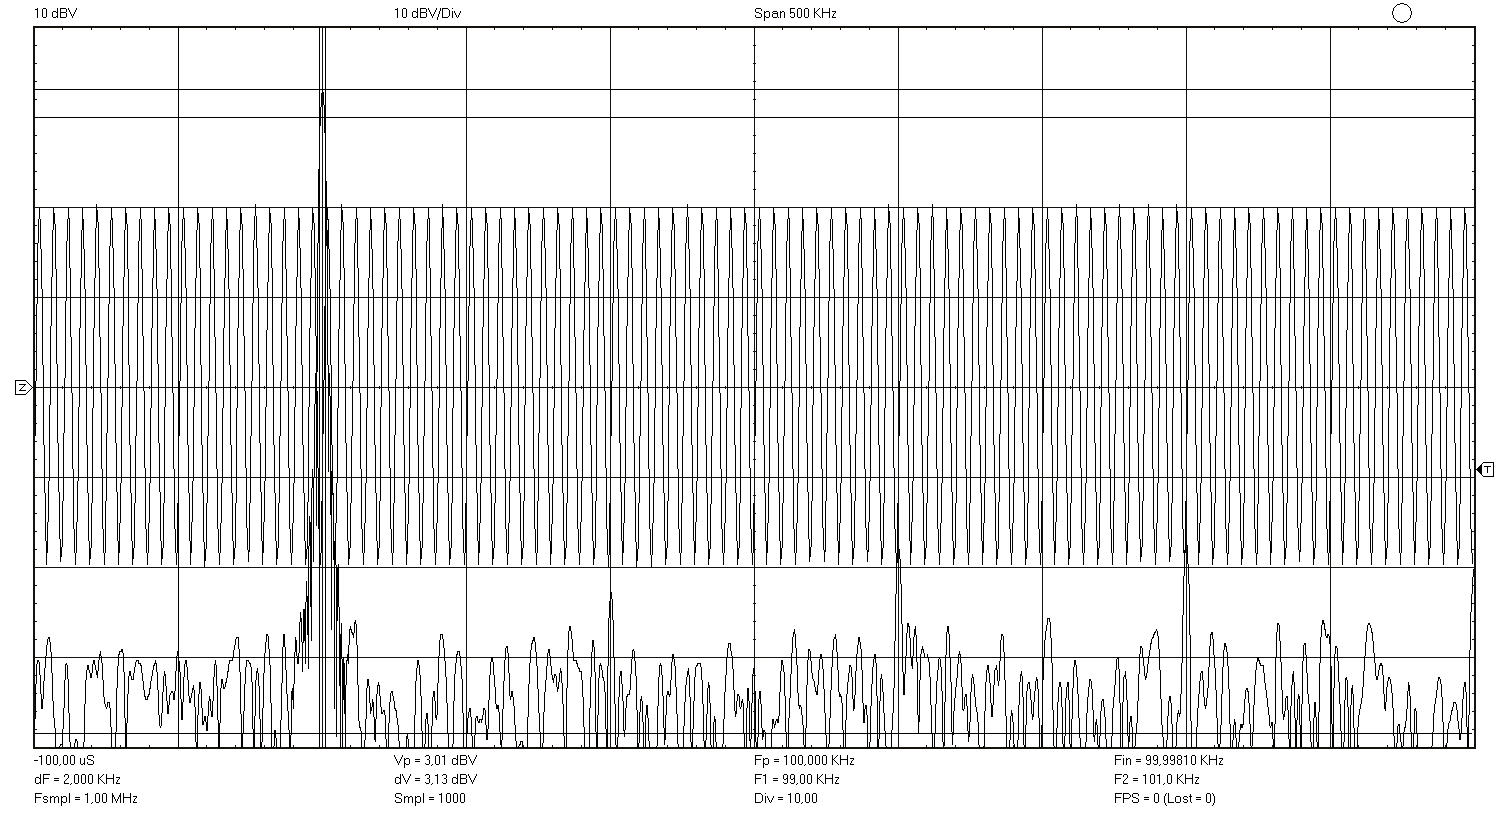
\includegraphics[width=.8\linewidth]{data/1-2_hanna_1MHZ}\hfill
\end{center}	
\begin{center}
	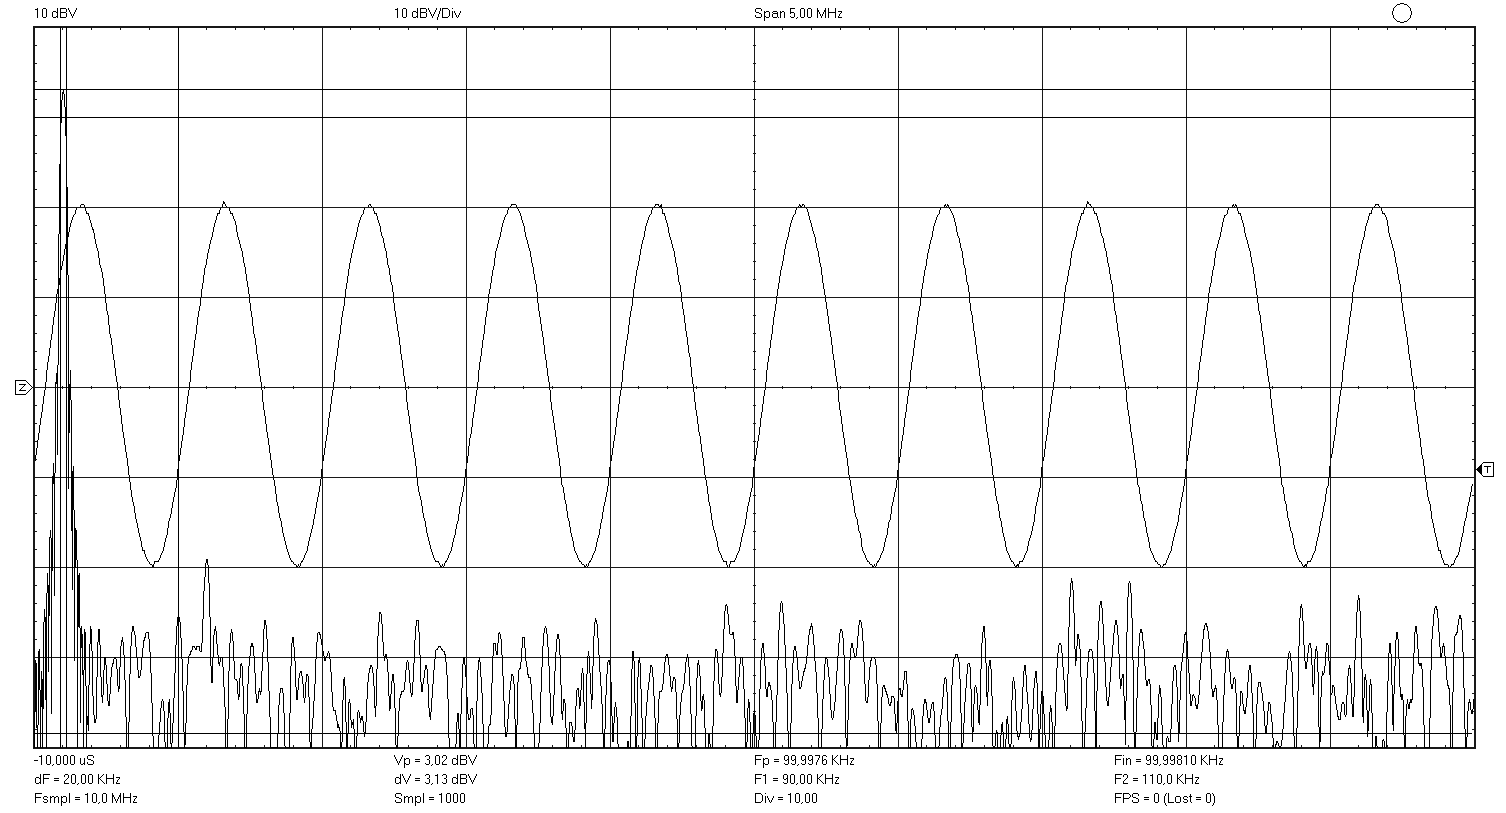
\includegraphics[width=.8\linewidth]{data/1-2_hanna_10MHZ}\hfill
\end{center}	
\begin{center}
	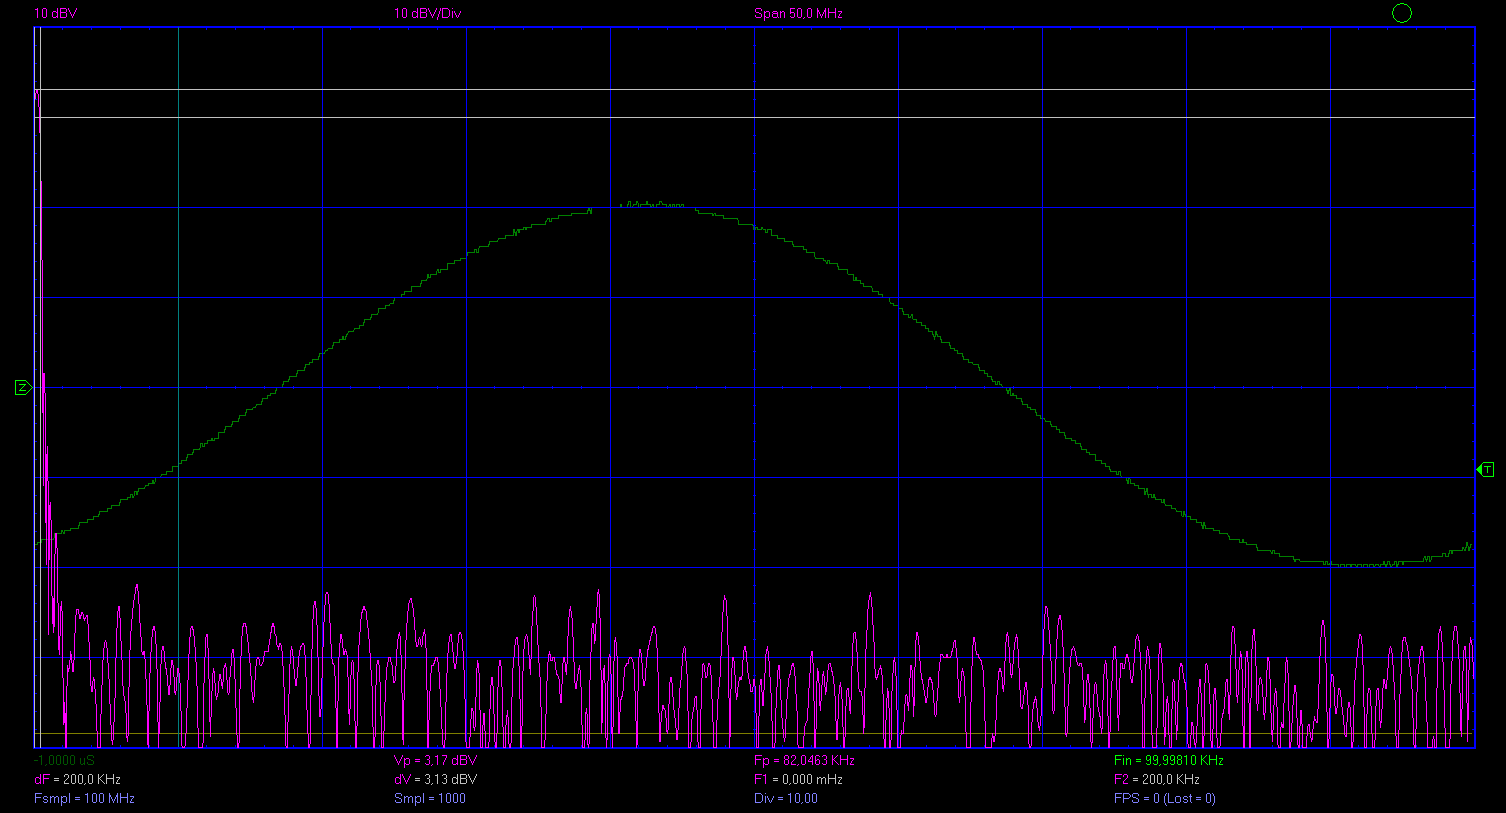
\includegraphics[width=.8\linewidth]{data/1-2_hanna_100MHZ}\hfill
\end{center}	

\subsection*{1.2. Спектр дискретизованной синусоиды (окно прямоугольное)}
\vspace*{20pt}

\begin{center}
	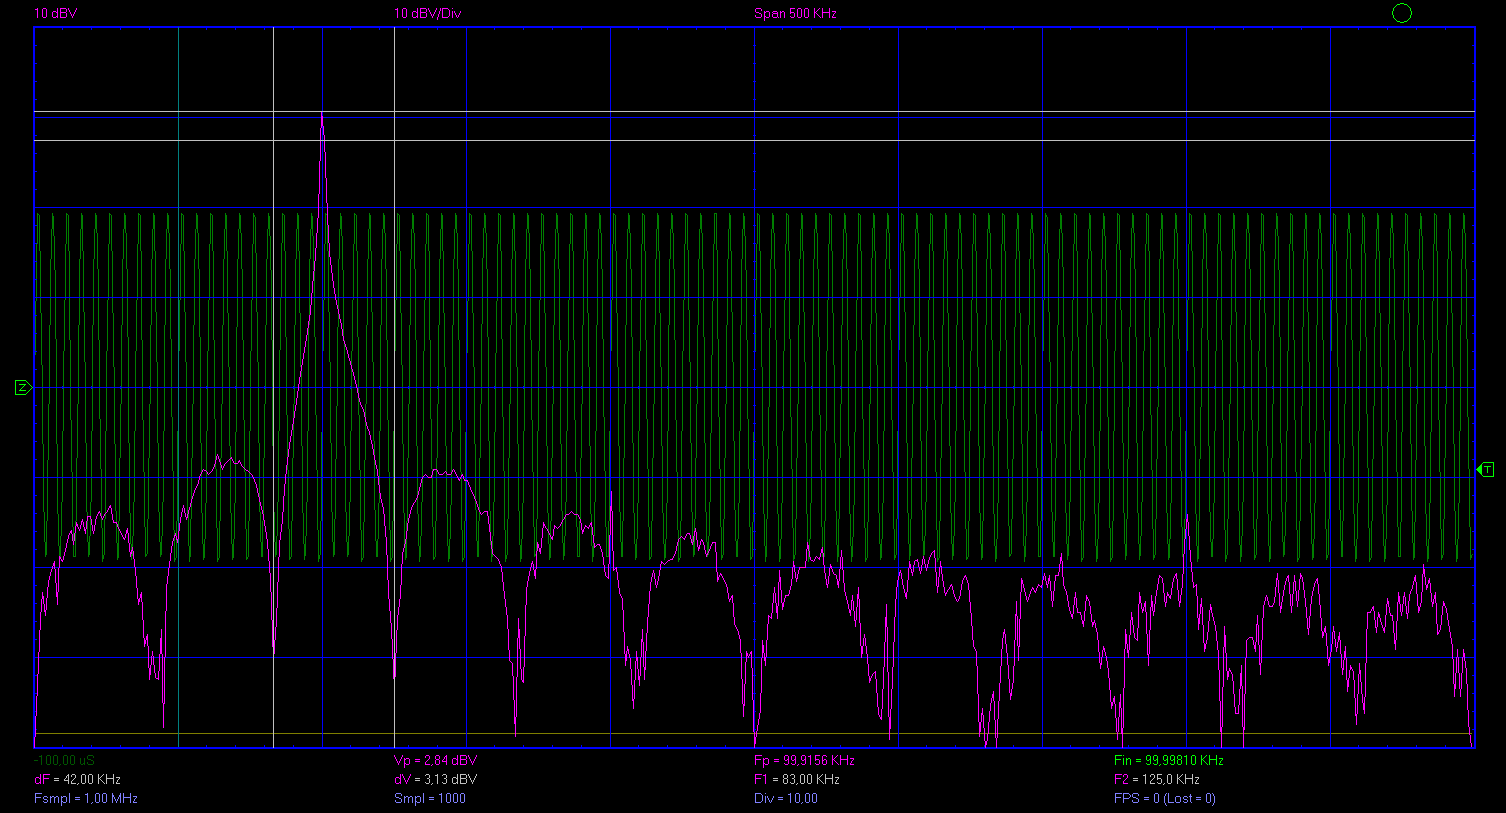
\includegraphics[width=.8\linewidth]{data/1-2_rect_1MHZ}\hfill
\end{center}	
\begin{center}
	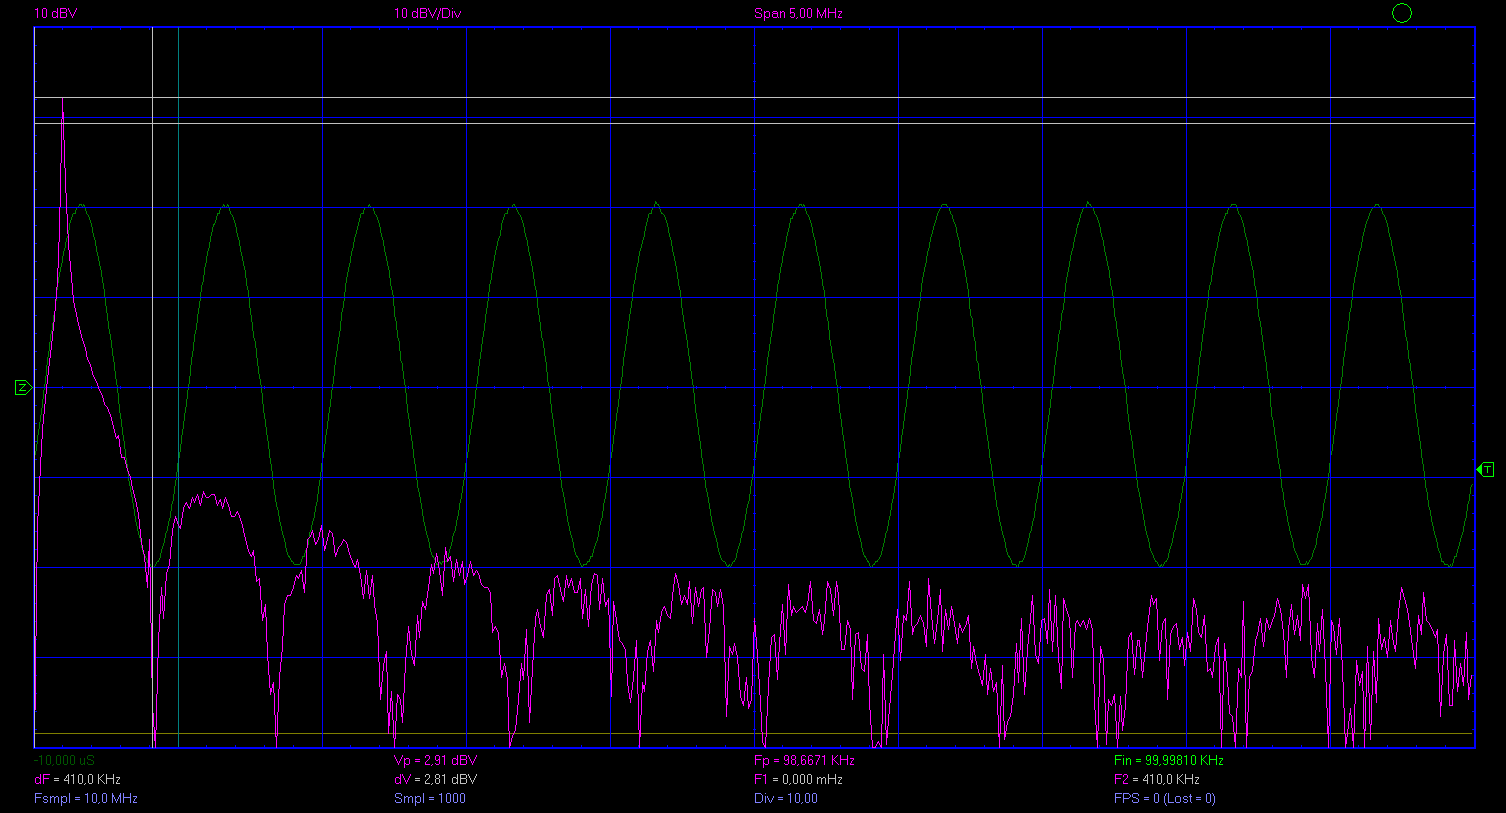
\includegraphics[width=.8\linewidth]{data/1-2_rect_10MHZ}\hfill
\end{center}	
\begin{center}
	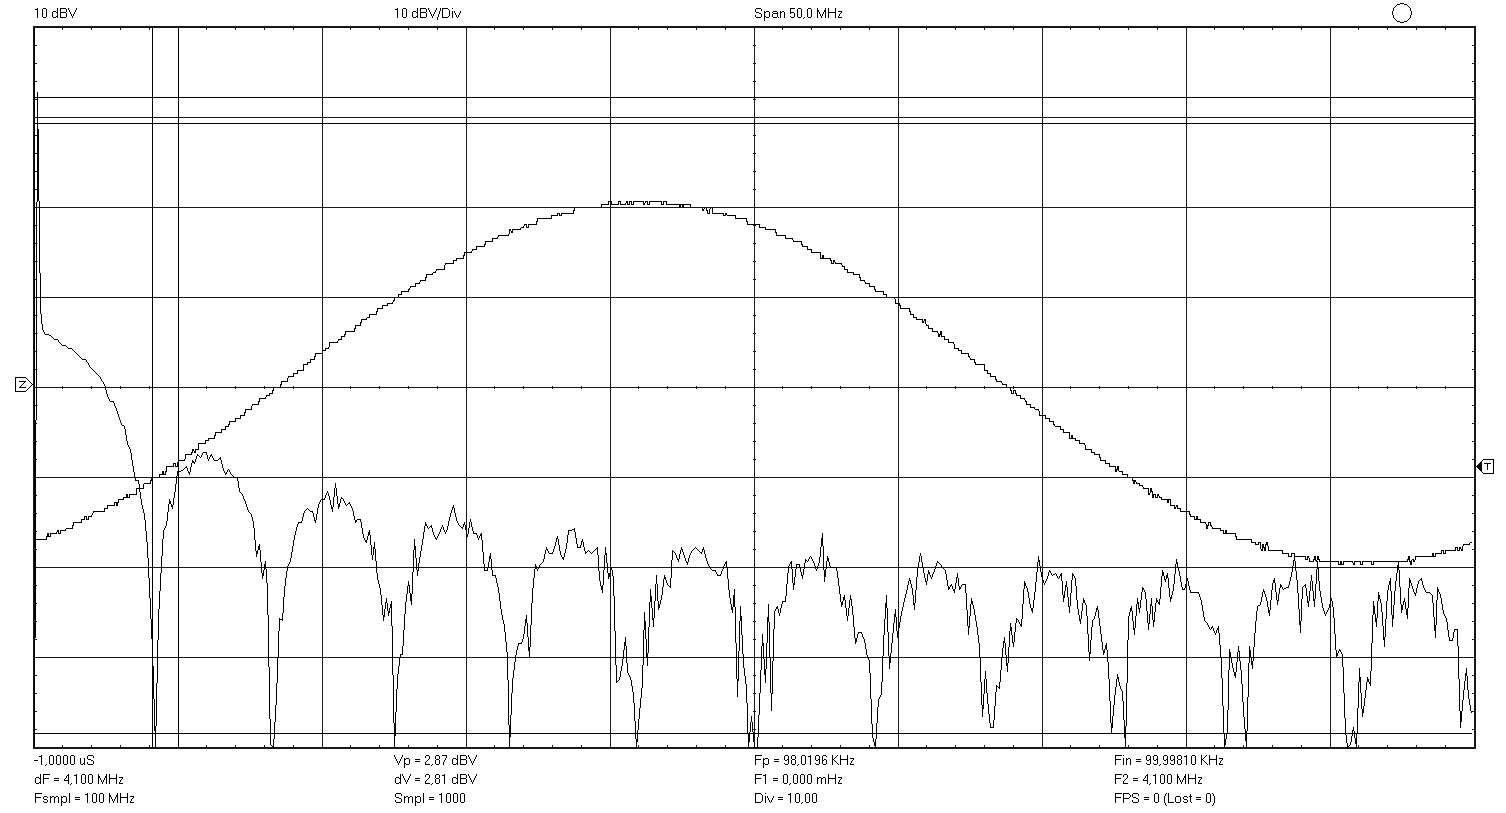
\includegraphics[width=.8\linewidth]{data/1-2_rect_100MHZ}\hfill
\end{center}	
\newpage

\subsection*{1.3. Эффект наложения (окно Ханна)}
\vspace*{20pt}

\begin{center}
	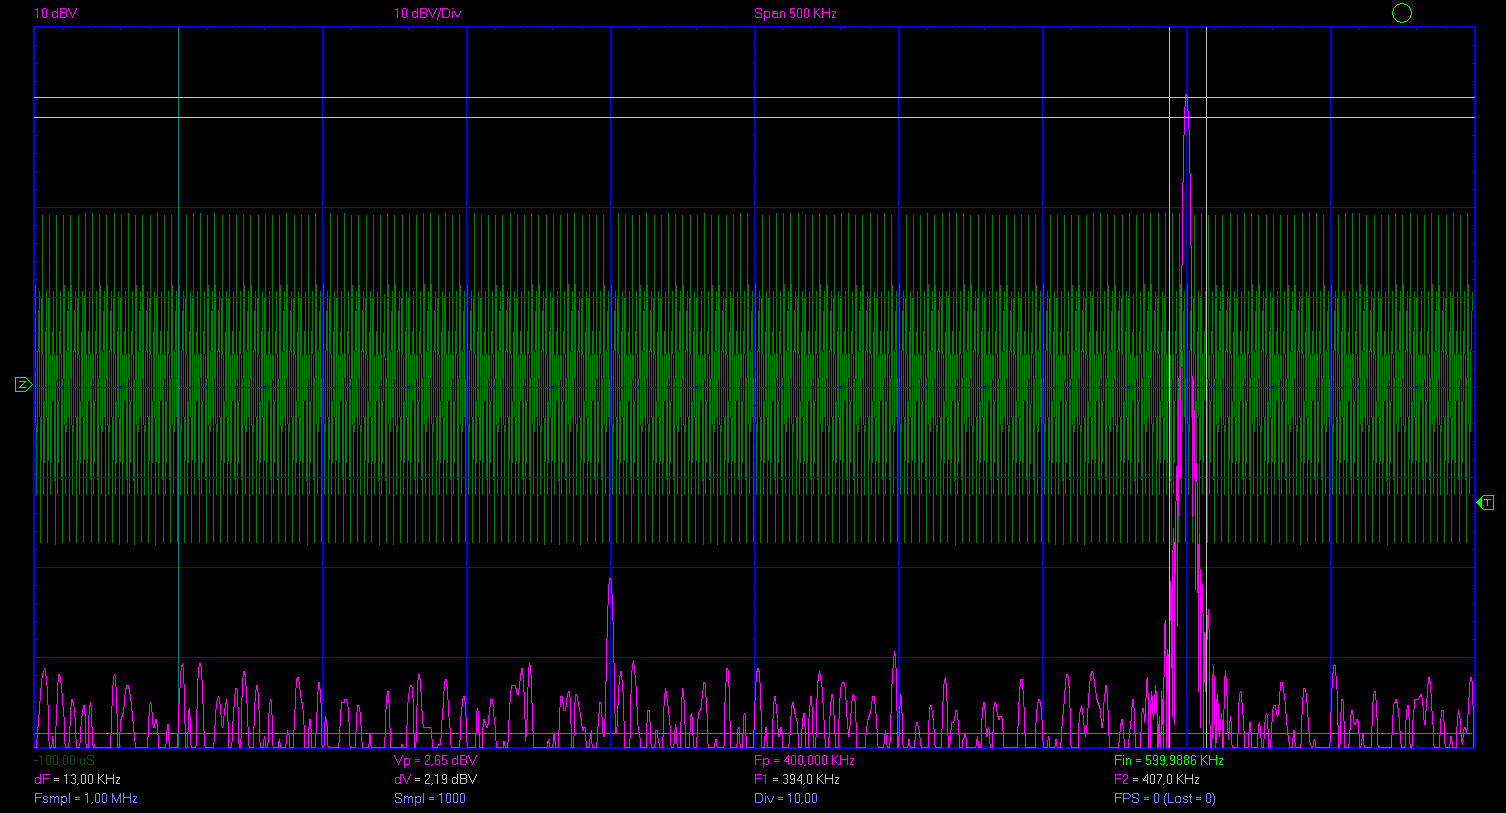
\includegraphics[width=.8\linewidth]{data/1-3_hanna_600KHZ}\hfill
\end{center}	
\begin{center}
	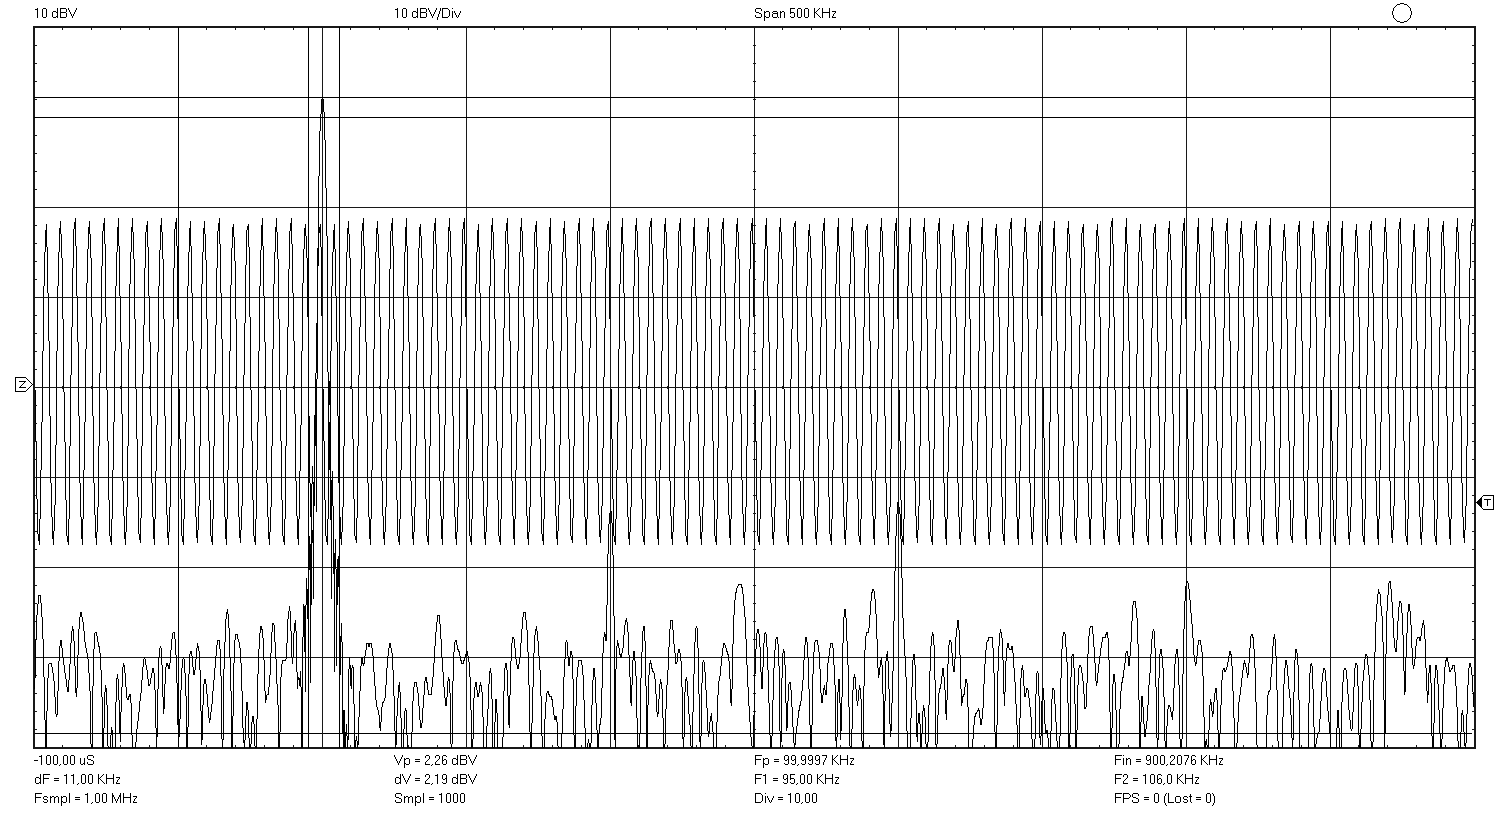
\includegraphics[width=.8\linewidth]{data/1-3_hanna_900KHZ}\hfill
\end{center}	

\newpage

\subsection*{1.3. Эффект наложения (окно прямоугольное)}
\vspace*{20pt}

\begin{center}
	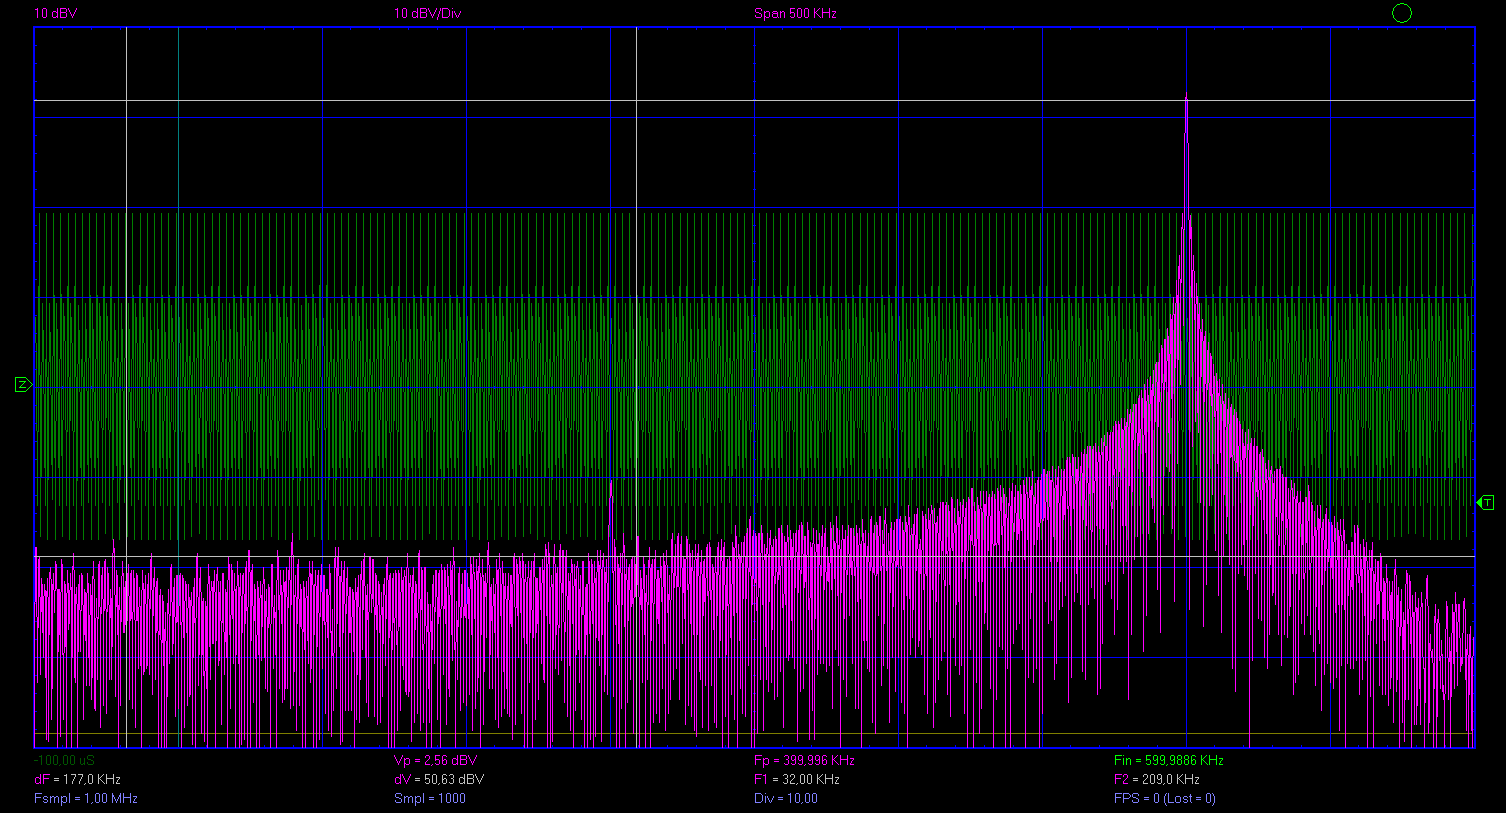
\includegraphics[width=.8\linewidth]{data/1-3_rect_600KHZ}\hfill
\end{center}	
\begin{center}
	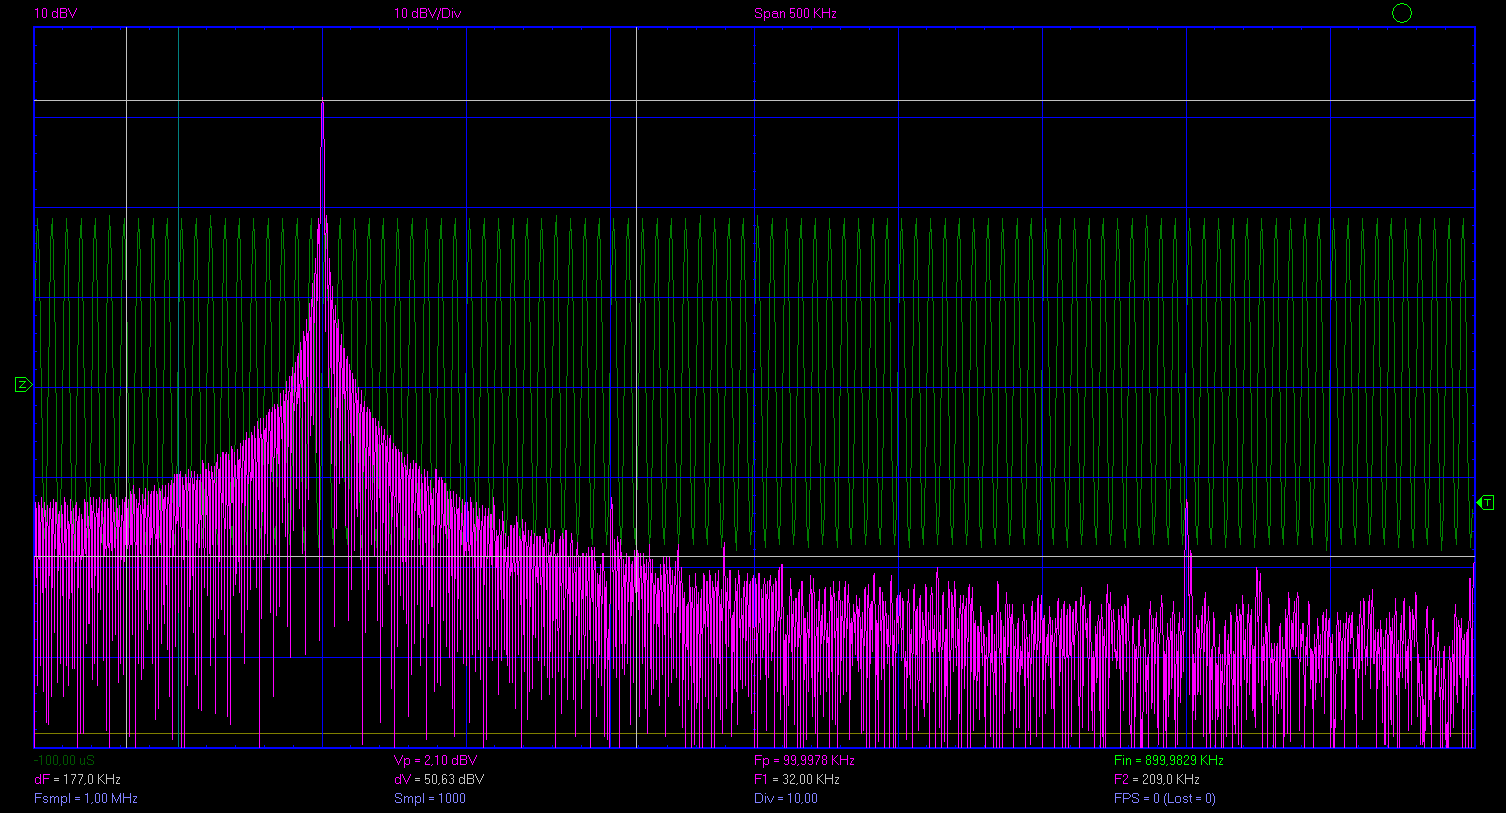
\includegraphics[width=.8\linewidth]{data/1-3_rect_900KHZ}\hfill
\end{center}	

\newpage



\section*{Субдискретизация полосовых радиосигналов}
\subsection*{Субдискретизация полосовых радиосигналов ($f_{\text{д}} = 100 \;\text{kHz}$)}
\vspace*{20pt}
\begin{center}
	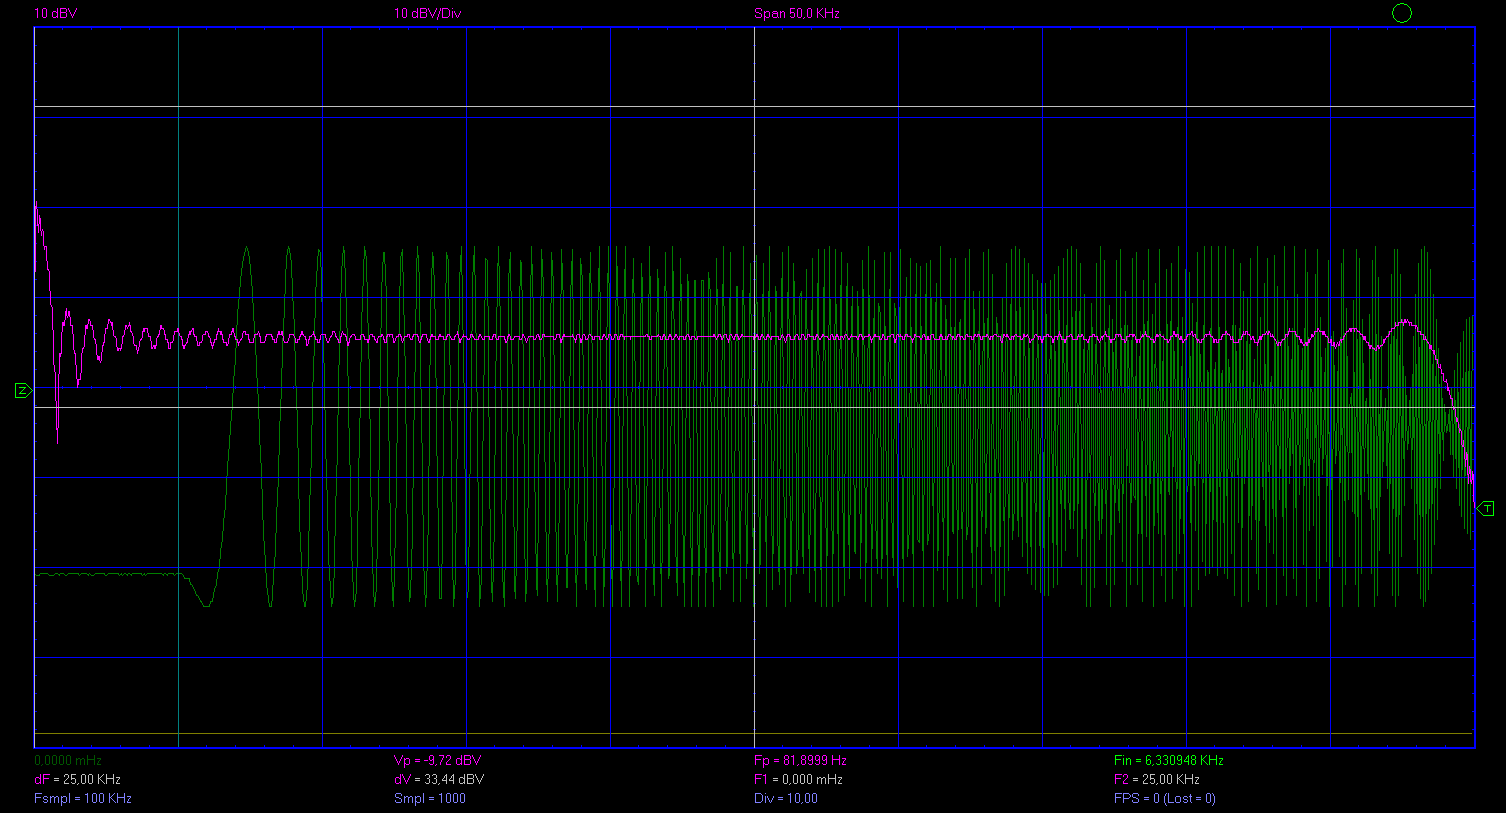
\includegraphics[width=.8\linewidth]{data/2-1_rect_0-50KHZ_100KHZ}\hfill
\end{center}	
\begin{center}
	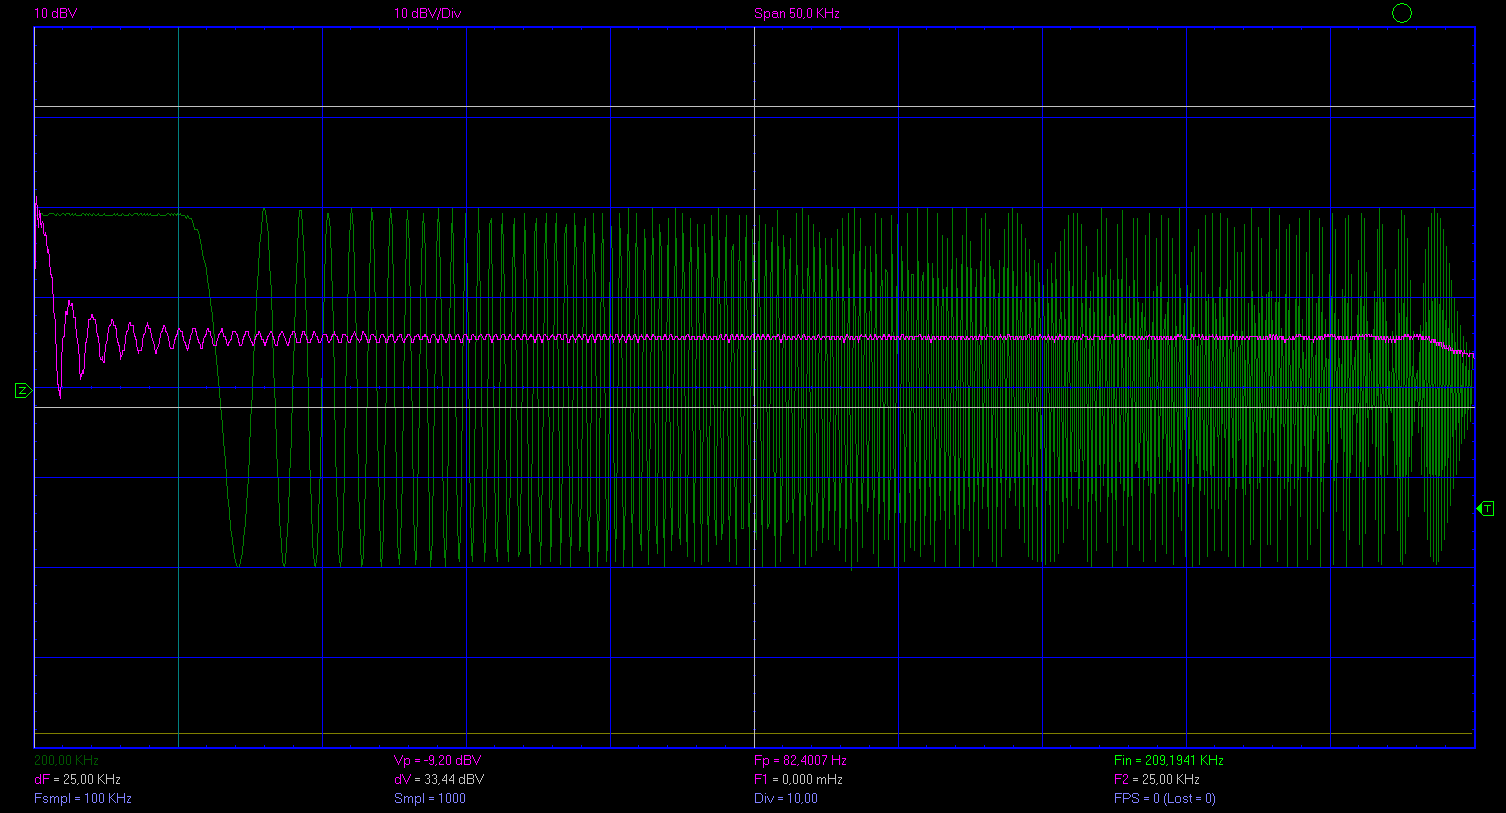
\includegraphics[width=.8\linewidth]{data/2-1_rect_200-250KHZ_100KHZ}\hfill
\end{center}	
\begin{center}
	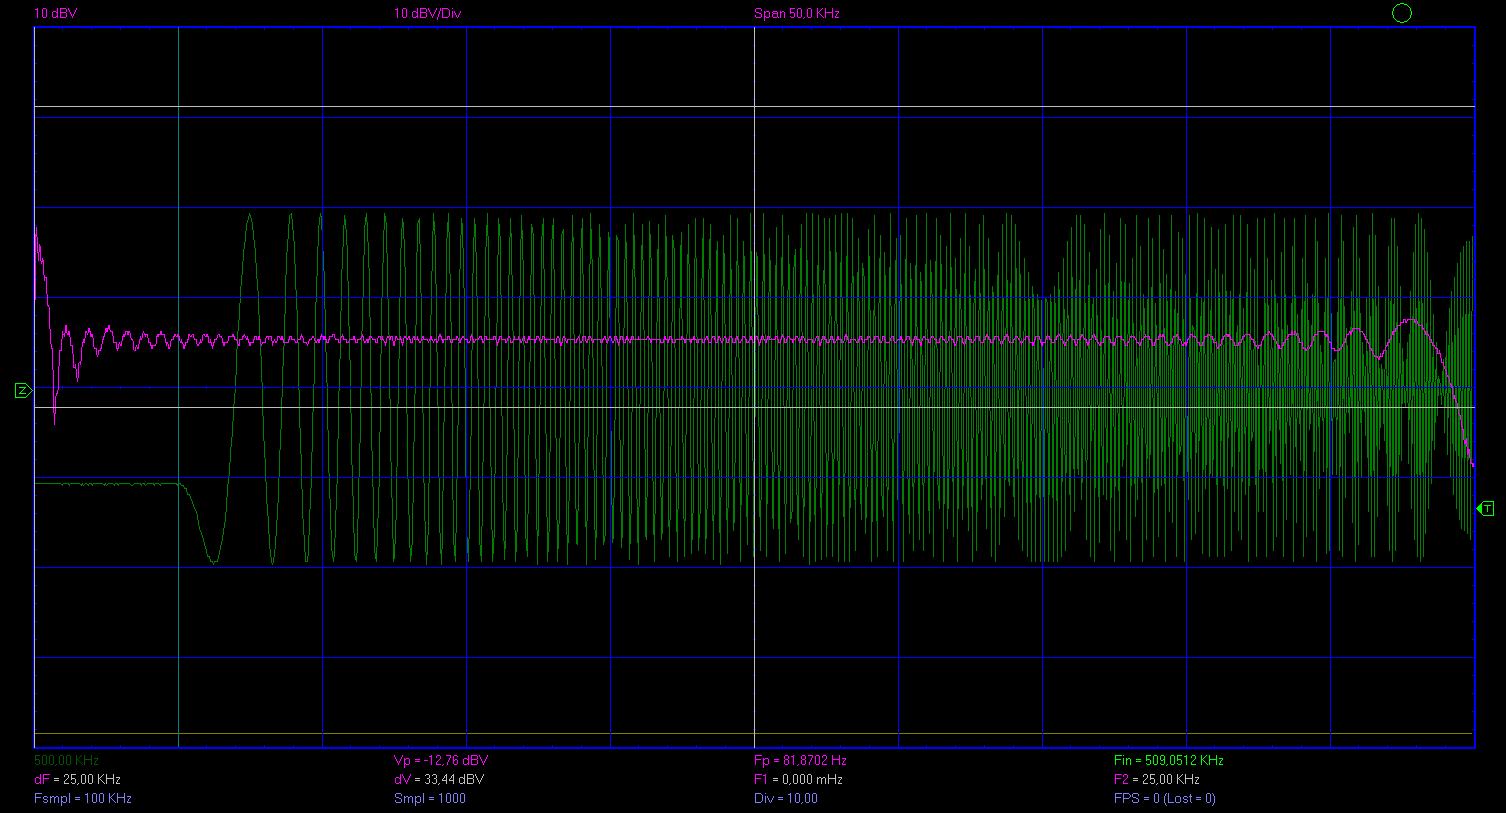
\includegraphics[width=.8\linewidth]{data/2-1_rect_500-550KHZ_100KHZ}\hfill
\end{center}	

\newpage

\subsection*{Субдискретизация полосовых радиосигналов ($f_{\text{д}} = 200 \;\text{kHz}$)}
\vspace*{20pt}
\begin{center}
	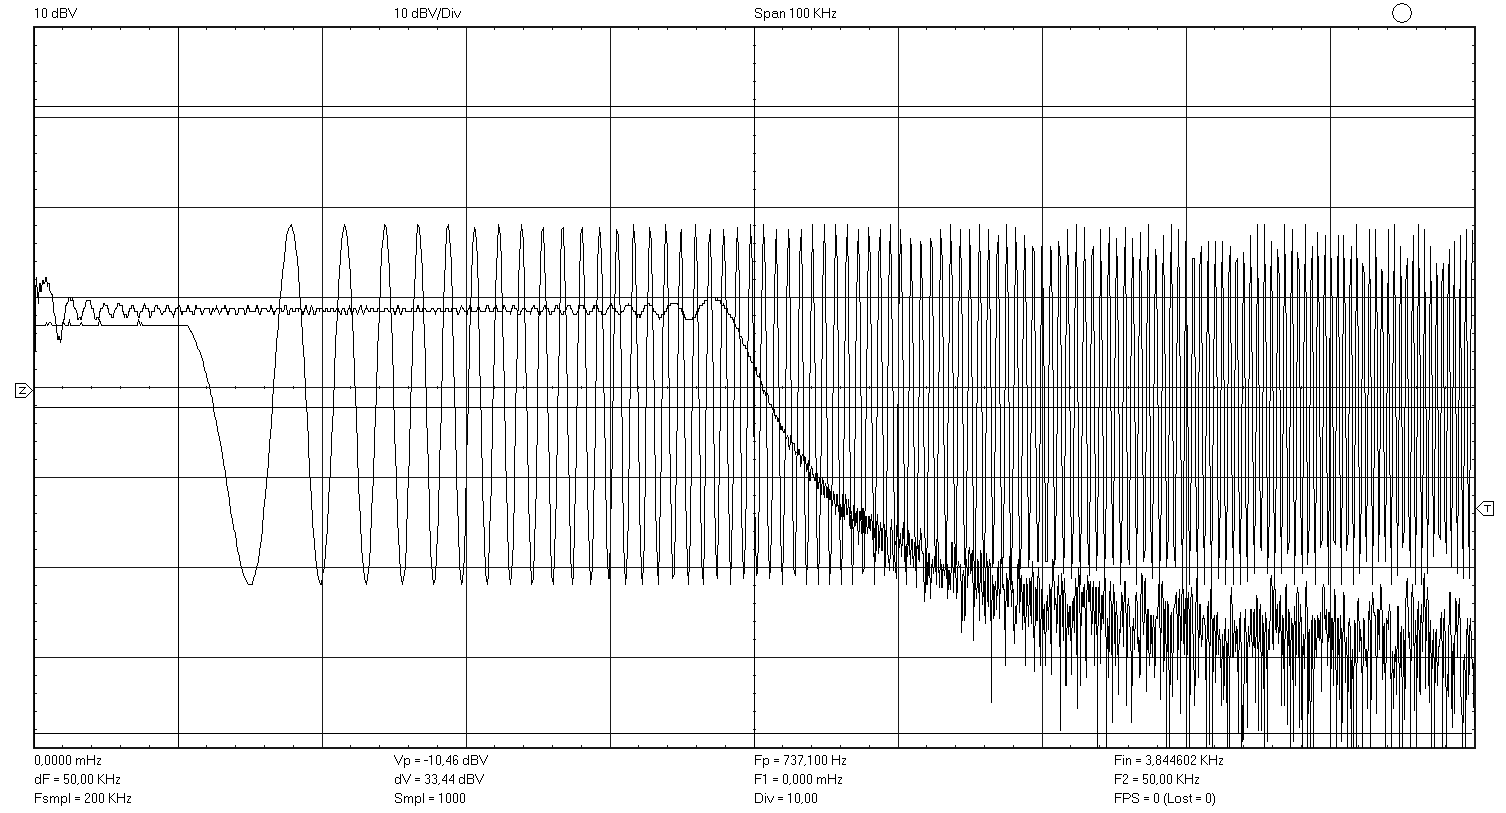
\includegraphics[width=.8\linewidth]{data/2-1_rect_0-50KHZ_200KHZ}\hfill
\end{center}	
\begin{center}
	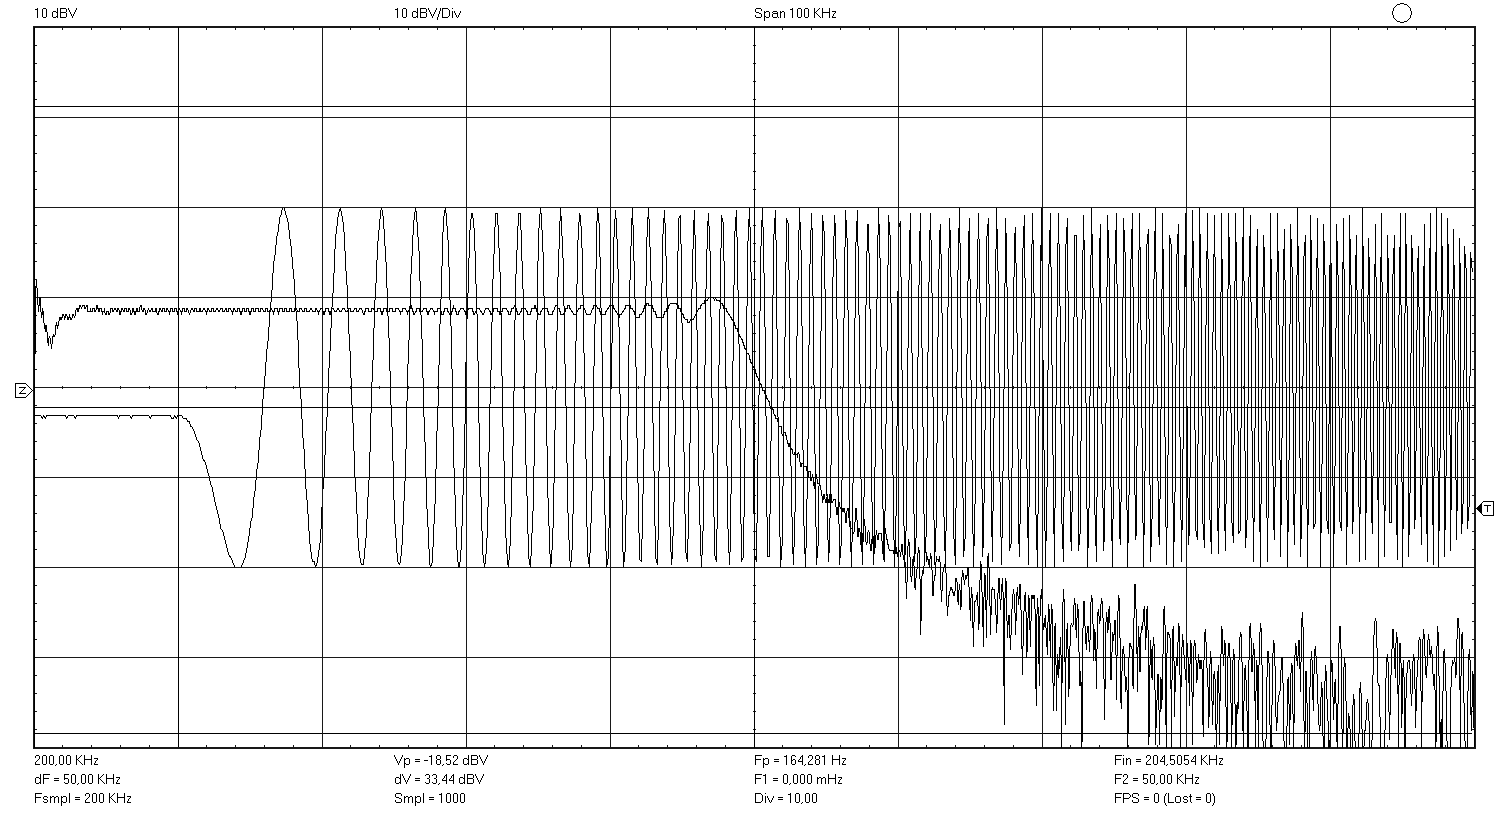
\includegraphics[width=.8\linewidth]{data/2-1_rect_200-250KHZ_200KHZ}\hfill
\end{center}	
\begin{center}
	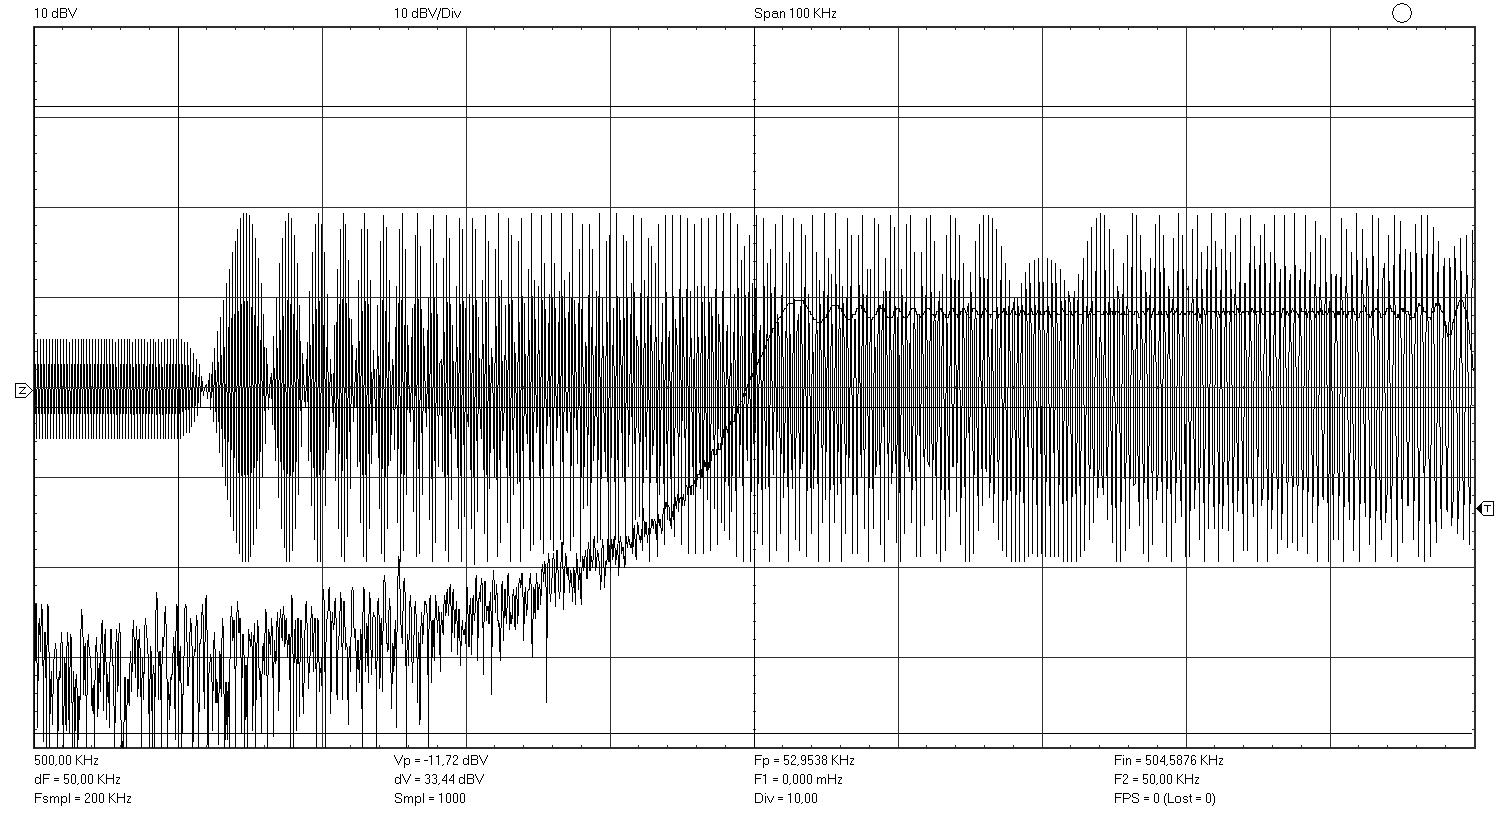
\includegraphics[width=.8\linewidth]{data/2-1_rect_500-550KHZ_200KHZ}\hfill
\end{center}	

\newpage


\subsection*{2.4 Выбор частоты дискретизации для нецелочисленных полос ($f_{\text{0}} = 998 \;\text{kHz}$  $f_{\text{в}} = 1 \;\text{kHz}$)}
\vspace*{20pt}
\begin{center}
	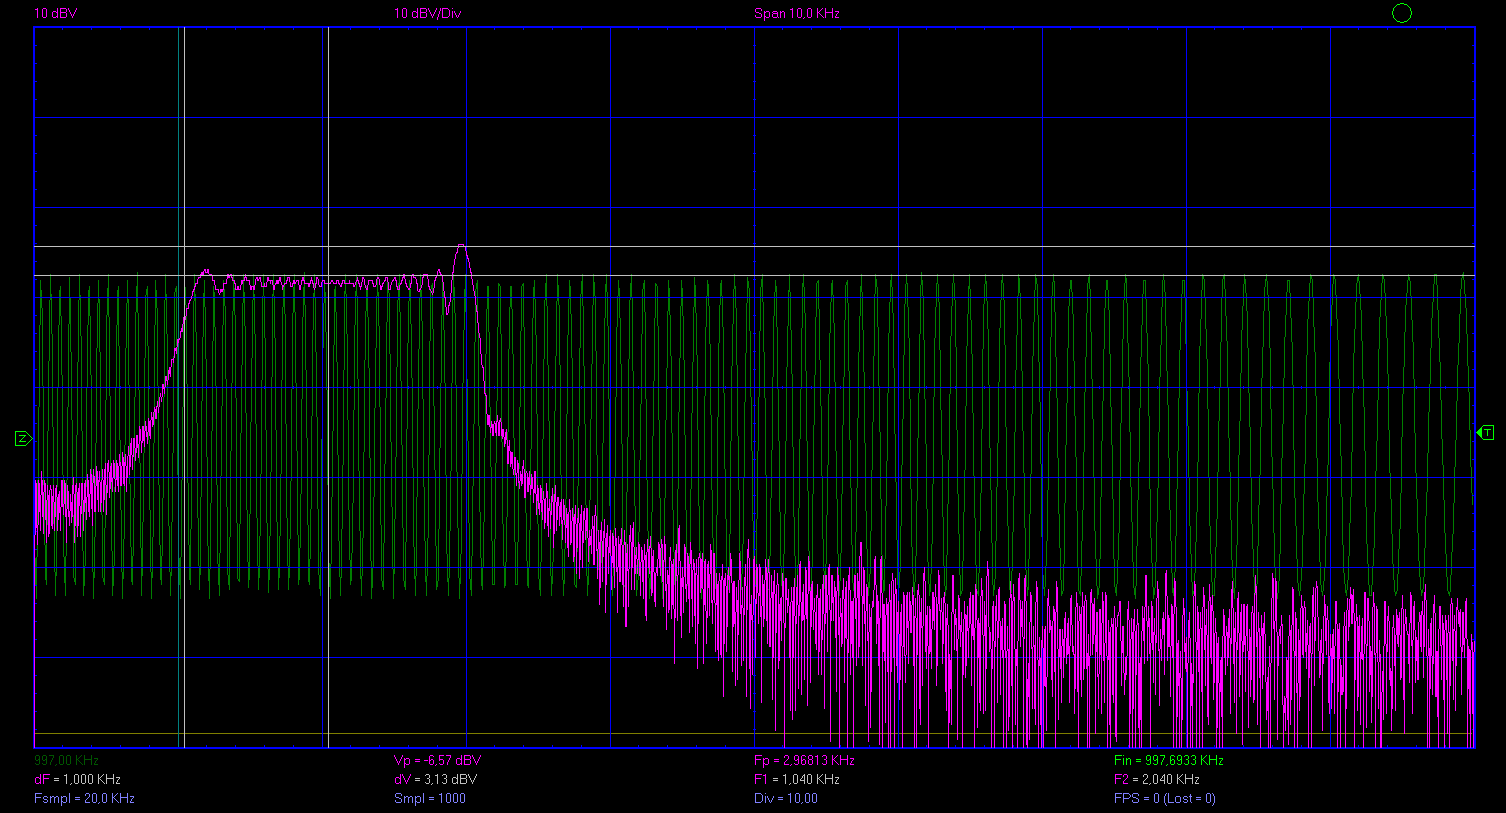
\includegraphics[width=1\linewidth]{data/2-4_rect_997KHZ-999KHZ_20KHZ}\hfill
\end{center}	

\newpage


\section*{Спектр дискретной последовательности прямоугольных импульсов}
\vspace*{20pt}

\subsection*{Спектрограммы (окно Ханна)}
\vspace*{20pt}
\begin{center}
	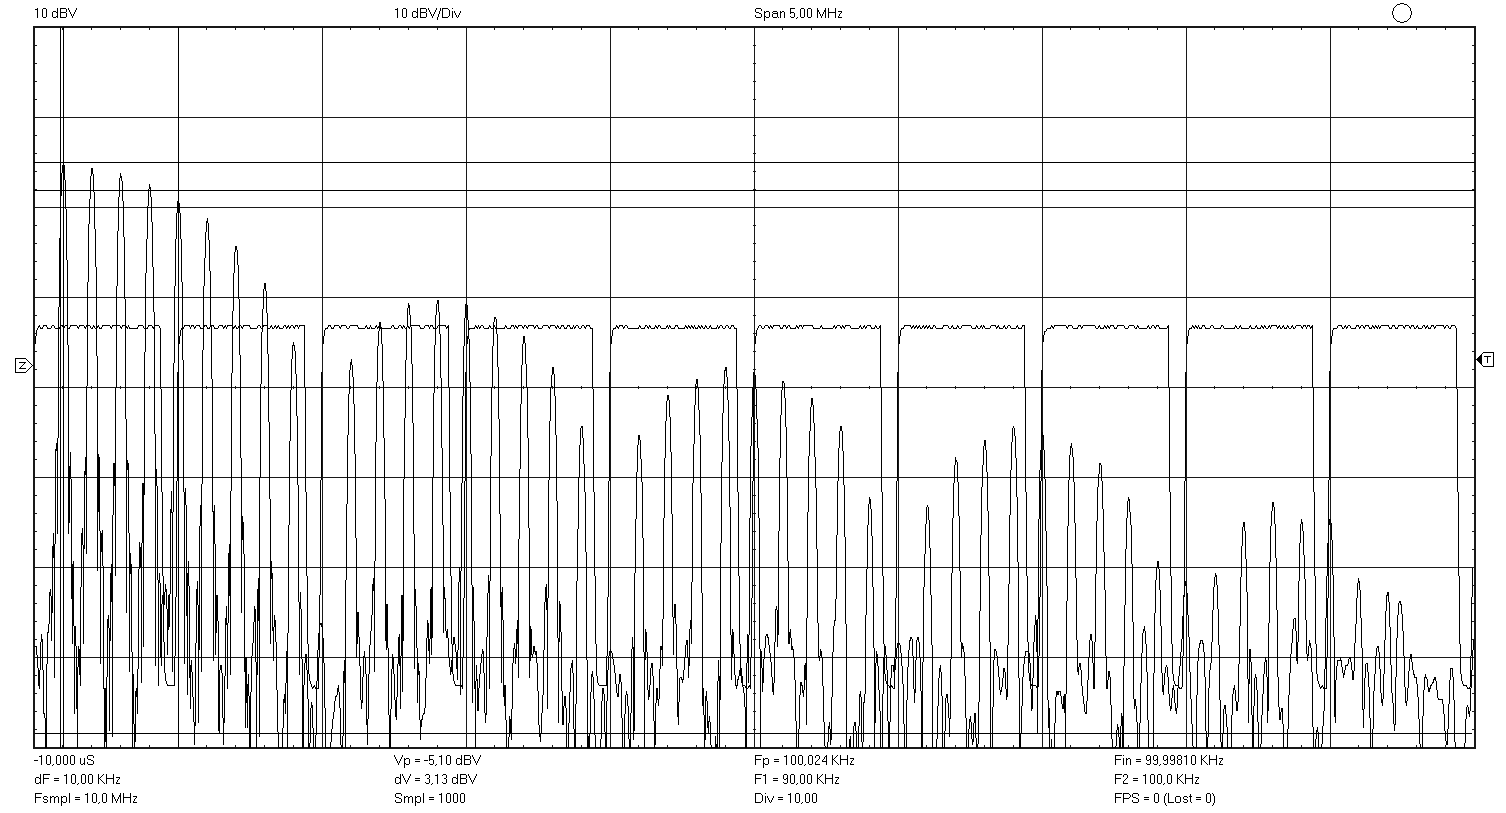
\includegraphics[width=.8\linewidth]{data/3-4_hanna_10MHZ_9mu-10mu}\hfill
\end{center}	
\begin{center}
	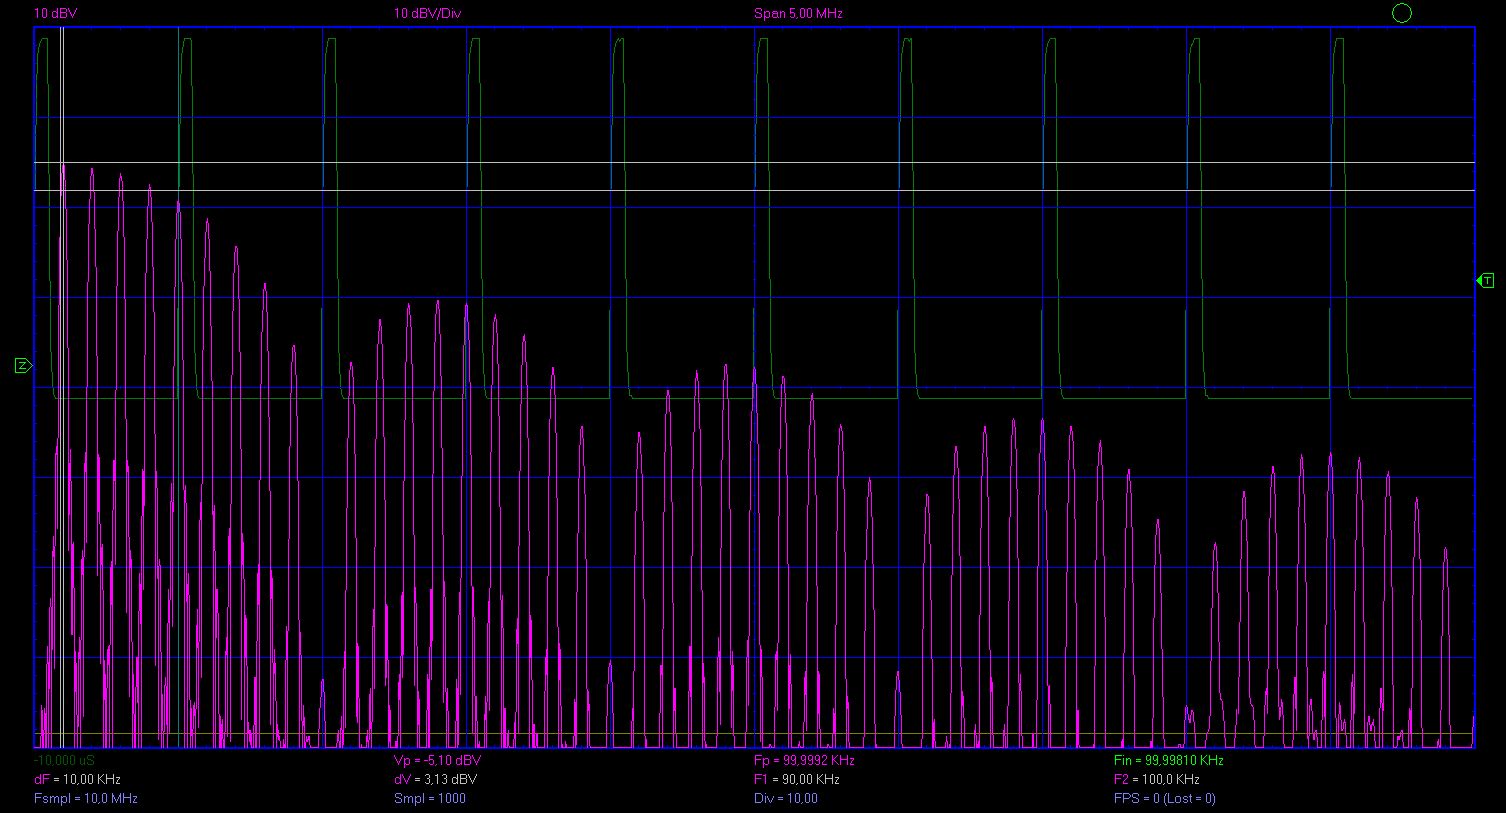
\includegraphics[width=.8\linewidth]{data/3-4_hanna_10MHZ_1mu-10mu}\hfill
\end{center}	

\newpage

\subsection*{Спектрограммы (окно прямоугольное)}
\vspace*{20pt}
\begin{center}
	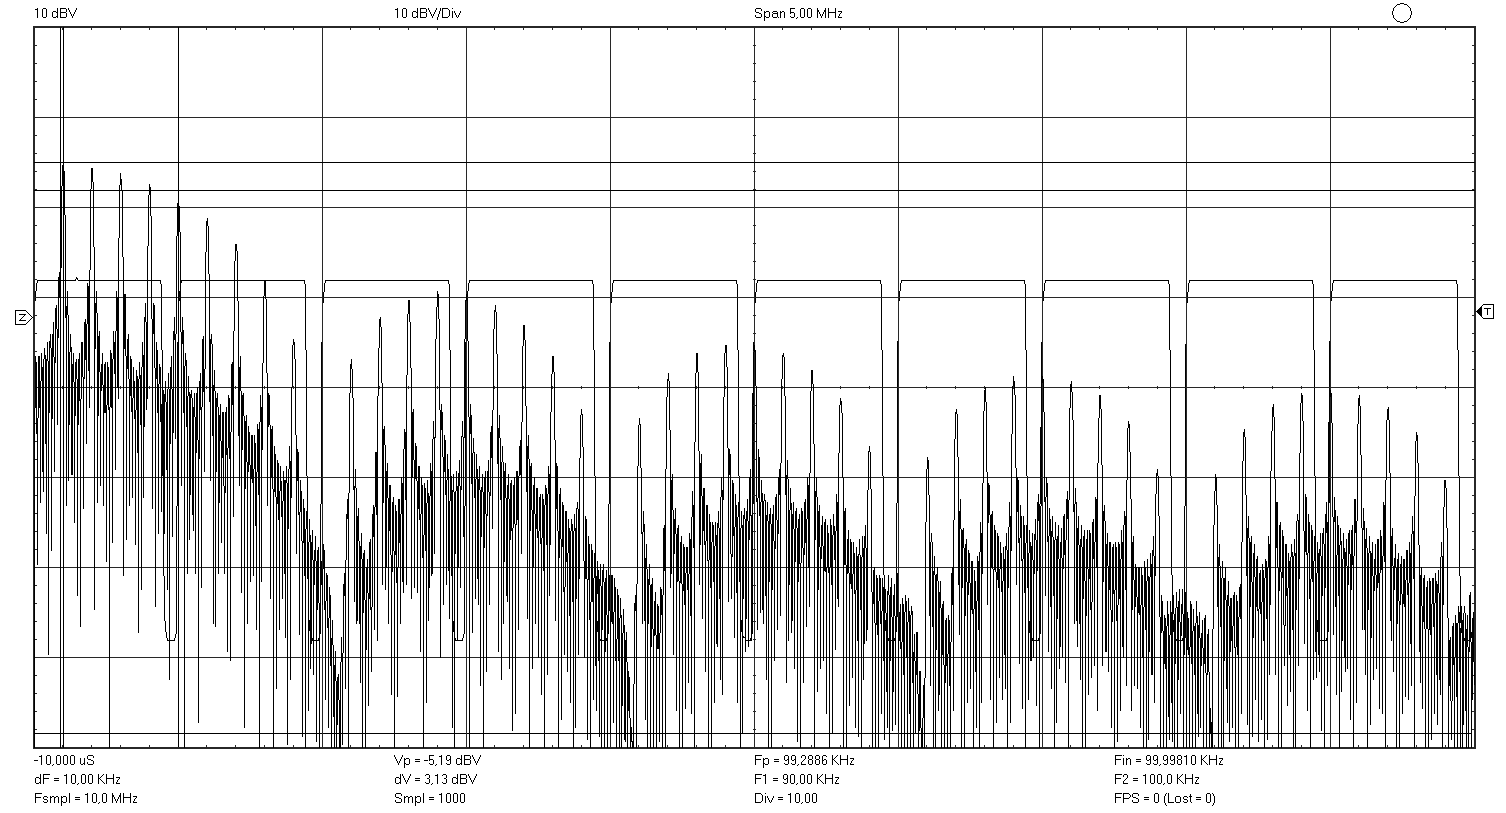
\includegraphics[width=.8\linewidth]{data/3-4_rect_10MHZ_9mu-10mu}\hfill
\end{center}	
\begin{center}
	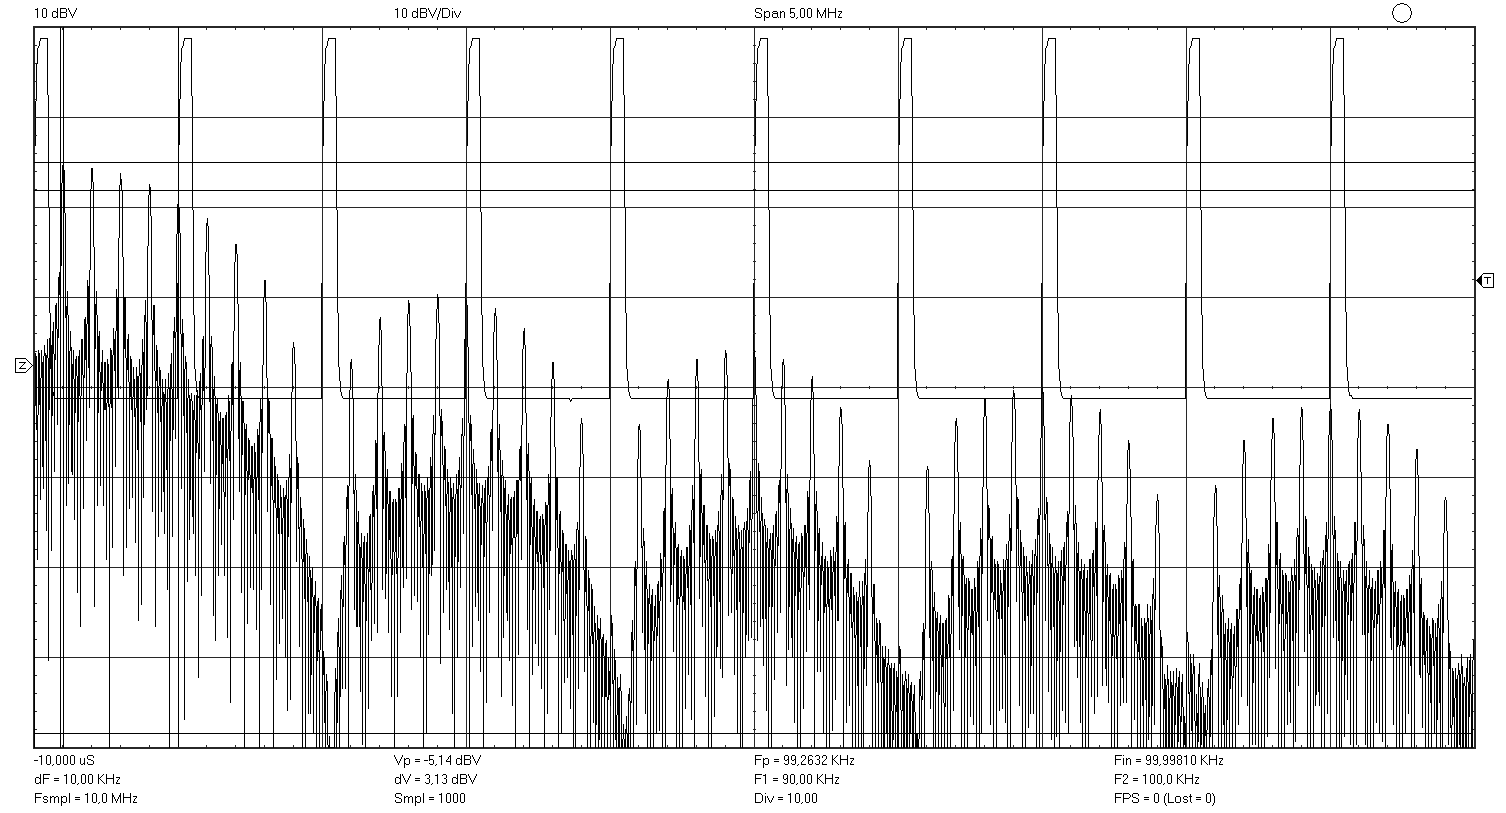
\includegraphics[width=.8\linewidth]{data/3-4_rect_10MHZ_1mu-10mu}\hfill
\end{center}	

\newpage

\end{document}
